\item
\begin{enumerate}
  \item Draw the Bayesian network clearly showing the nodes and arrows showing relationship among all the variables.
        \begin{center}
          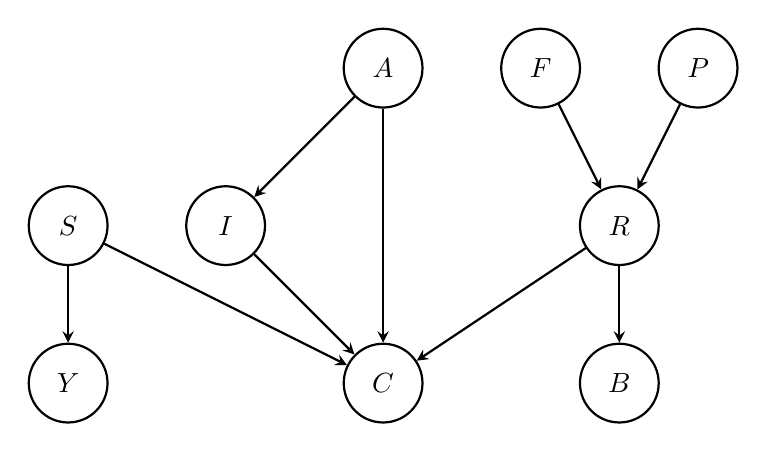
\begin{tikzpicture}[->,>=stealth,auto,node distance=0cm,
              thick,main node/.style={circle,draw}, minimum size=1cm]

            \node[main node] (S) at (0,2) {$S$};
            \node[main node] (Y) at (0,0) {$Y$};
            \node[main node] (I) at (2,2) {$I$};
            \node[main node] (A) at (4,4) {$A$};
            \node[main node] (C) at (4,0) {$C$};
            \node[main node] (F) at (6,4) {$F$};
            \node[main node] (R) at (7,2) {$R$};
            \node[main node] (B) at (7,0) {$B$};
            \node[main node] (P) at (8,4) {$P$};

            \path[every node/.style={}]
            (S) edge (Y)
            (S) edge (C)
            (A) edge (I)
            (A) edge (C)
            (I) edge (C)
            (F) edge (R)
            (P) edge (R)
            (R) edge (C)
            (R) edge (B);
          \end{tikzpicture}
        \end{center}
\end{enumerate}